\documentclass[10pt, fleqn]{article}
\usepackage[a4paper,margin=0.5in]{geometry}
\usepackage{multicol}
\usepackage{amsmath, amssymb}
\usepackage{titlesec}
\usepackage{float}
\usepackage{amsfonts, bm, graphicx}
\setlength{\mathindent}{0pt} % remove indent for equations

\titleformat{\section}{\large\bfseries}{}{0em}{}
\titleformat{\subsection}{\normalsize\bfseries}{}{0em}{}

\begin{document}

\begin{center}
    \Large \textbf{Dynamics Formula Sheet} \\
    \normalsize Quiz I
\end{center}

\begin{multicols}{2}

\section*{Kinematics}
\[\vec{v}=\frac{dx}{dt}\]
\[\vec{a}=\frac{d\vec{v}}{dt}=\frac{d\vec{x}}{dt}\]
\underline{Note:} Using the chain rule, $\vec{a}$ can be rewritten
\[\vec{a}=\vec{v}\frac{d\vec{x}}{dt}\]
\section*{Constant Acceleration Kinematics}
\[\vec{v}=\vec{v}_o+\vec{a}_ot\]
\[\vec{v}_f^2=\vec{v}_o^2+2\vec{a}_o\Delta \vec{x}\]
\[\vec{x}=\vec{x}_o+\vec{v}_ot+\frac{1}{2}\vec{a}_ot^2\]
\section*{Relative Motion}
\[x_{B/A}=x_B-x_A \quad \text{B relative to A}\]
\underline{Note:} Subscripts cancel $x_B=x_A+x_{B/A}$
\section*{Normal and Tangential}
\begin{figure}[H]
    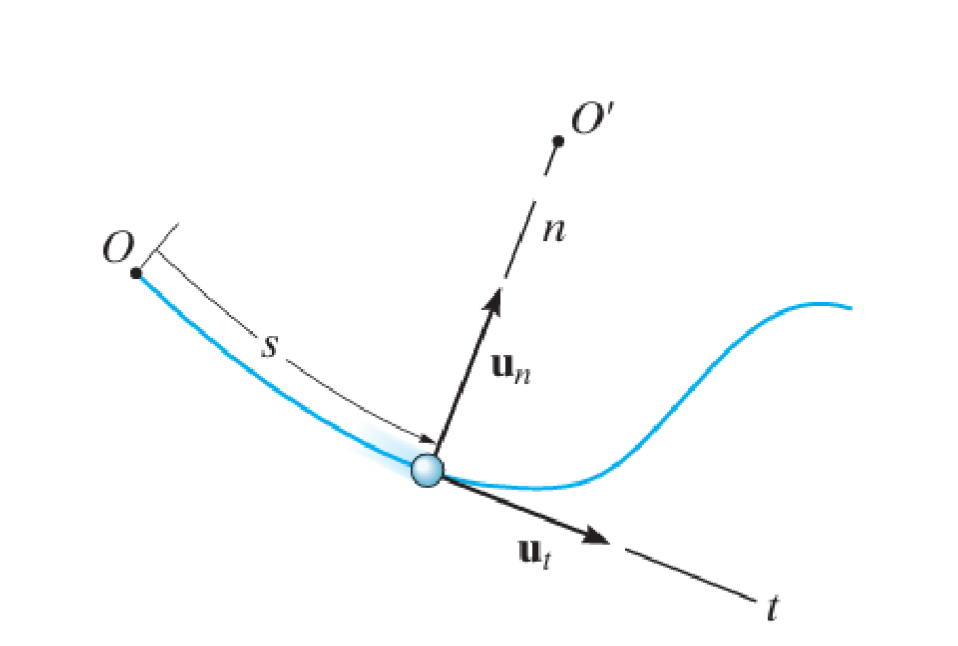
\includegraphics[width=0.3\textwidth]{normal and tangential.png}
\end{figure}
\[\vec{v}=v\hat{u}_t\]
\[\vec{a}=\frac{dv}{dt}\hat{u}_t+\frac{v^2}{\rho}\hat{u}_n\]
\[\rho = \frac{\left[1+\left(\frac{dy}{dx}\right)^2 \right]^{3/2}}{\left|\frac{d^2y}{dx^2} \right|} \quad \text{(Radius of curvature)}\]
\underline{Note:} In 3d, define $\hat{u}_b=\hat{u}_t \times \hat{u}_n$ 
\columnbreak
\section*{Cylindrical (Radial and Transverse)}
\begin{figure}[H]
    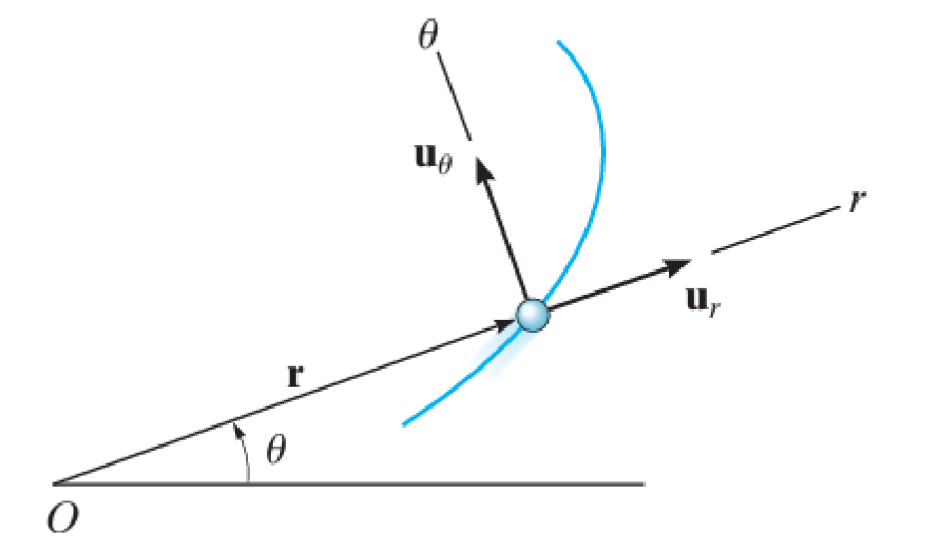
\includegraphics[width=0.3 \textwidth]{cylindrical.png}
\end{figure}
\[\vec{v}=\dot{r}\hat{u}_r+r\dot{\theta}\hat{u}_{\theta}\]
\[\vec{a}=\left[\ddot{r}-r\dot{\theta}^2\right]\hat{u}_r+\left[r\ddot{\theta}+2\dot{r}\dot{\theta}\right]\hat{u}_{\theta}\]
\underline{Note:} In 3d, add a $\hat{u}_z$ where $\vec{r}_z=z\hat{u}_z$,$\vec{v}_z=\dot{z}\hat{u}_z$ and $\vec{a}_z=\ddot{z}\hat{u}_z$
\begin{figure}[H]
    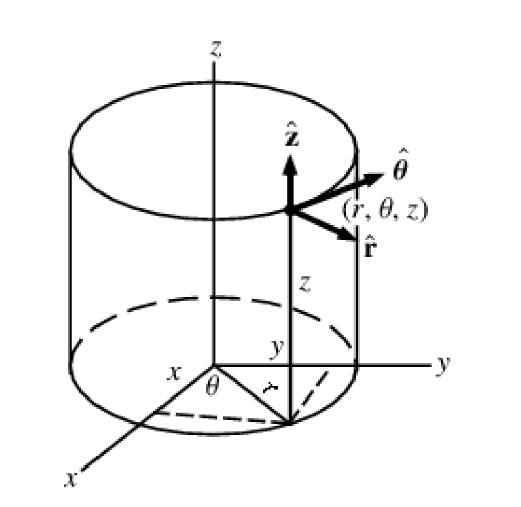
\includegraphics[width=0.3 \textwidth]{3d cylindrical.png}
\end{figure}
\end{multicols}
\newpage
\makeatletter
\@fleqnfalse
\makeatother

\begin{center}
    \Large \textbf{Orbital Mechanics}
\end{center}
\section*{Newton's Law of Gravitation}
\[F_g=\frac{GMm}{r^2}\]
\section*{Differential equation (for shape of orbital trajectory):}
Derived by applying \textbf{central force motion} 
\begin{figure}[H]
    \centering
    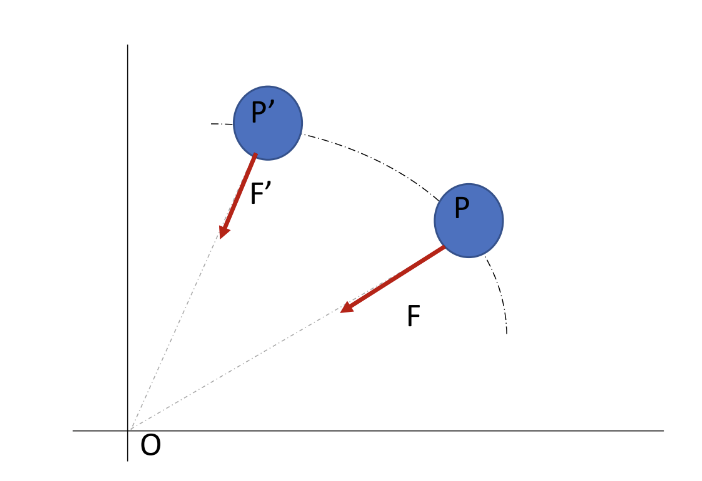
\includegraphics[width=0.3\textwidth]{central force.png}    
\end{figure}
\noindent
\[\begin{array}{rcl@{\hskip 1.2cm}rcl}
\sum F_r &=& ma_r & \sum F_\theta &=& ma_\theta \\
-F &=& m(\ddot{r} - r\dot{\theta}^2) & 0 &=& m(r\ddot{\theta} + 2\dot{r}\dot{\theta})
\end{array}\]\\\\
Rewriting $-F = m(\ddot{r} - r\dot{\theta}^2)$ only in terms of $\theta$ using $h=r^2\dot{\theta}$:
\begin{center}
\boxed{\frac{d^2u}{d\theta^2} + u = \frac{GM}{h^2}}
\end{center}
Where:
\begin{itemize}
    \item $u=1/r$, r is distance from centers of mass 
    \item $h=r^2\dot{\theta}$ , angular momentum per unit mass (where angular momentum $=H_o=hm=rmv_\theta$ )
    \item $G=6.67\times10^{-11} m^3/kgs^2$
    \item M is the mass of the central body
\end{itemize}
\section*{Solutions to this differential equation are conic paths:} 
\begin{figure}[H]
    \centering
    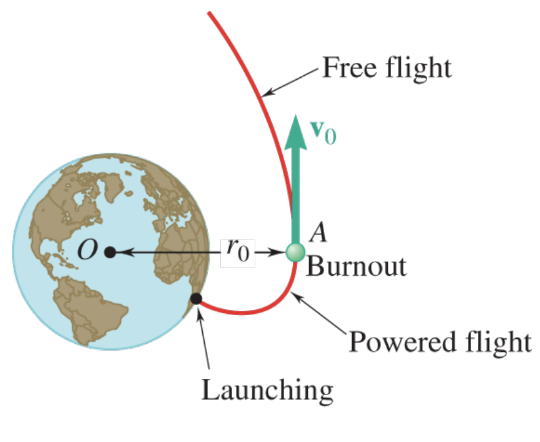
\includegraphics[width=0.3\textwidth]{orbital.png}
\end{figure}
\begin{center}
\boxed{u = \frac{1}{r} = \frac{GM}{h^2} + C\cos\theta = \frac{GM}{h^2}(1 + \varepsilon\cos\theta)}
\end{center}
Where C and h are constants defined by the instantaneous r and v at any point along the orbit:
\begin{itemize}
    \item $h =  r^2\dot{\theta} = r_0v_0$ 
    \item $C = \frac{1}{r_0} - \frac{GM}{h^2} = \frac{1}{r_0} - \frac{GM}{r_0^2v_0^2}$
\end{itemize}
\newpage \noindent
With \textbf{eccentricity}:
\[\varepsilon = \frac{C}{GM/h^2} = \frac{Ch^2}{GM}\]
\underline{Note:} 
\begin{multicols}{2}
\begin{figure}[H]
    \centering
    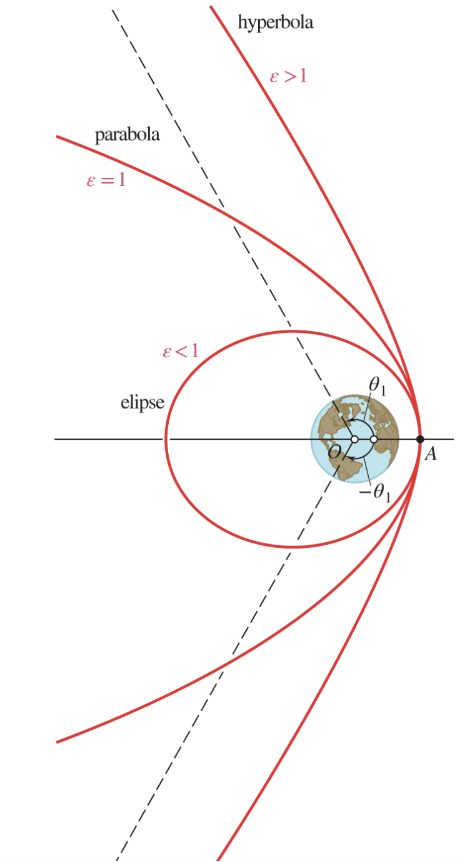
\includegraphics[width=0.3\textwidth]{eccentricity.png}
\end{figure}
\begin{align*}
&\varepsilon > 1: \quad \text{Hyperbola} \\
&\varepsilon = 1: \quad \text{Parabola} \\
&\varepsilon < 1: \quad \text{Ellipse} \\
&\varepsilon = 0: \quad \text{Circle}
\end{align*}
\end{multicols}
\section*{Initial conditions for each path}
\begin{figure}[H]
    \centering
    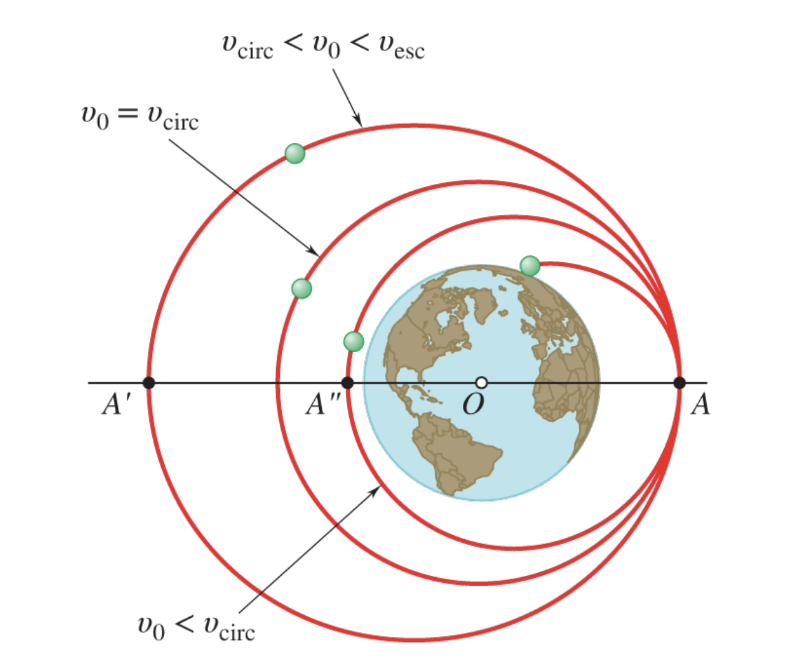
\includegraphics[width=0.4\textwidth]{conditions.png}
\end{figure}
\textbf{Parabolic path (barely escaping orbit) $\varepsilon =1$:}
\[u = \frac{1}{r} = \frac{GM}{h^2}(1 + \cos\theta)\]
At $\theta=0$ and $r=r_o$ (at start of free flight):
\[\frac{1}{r_o} = \frac{GM}{r_o^2v_o^2}(1 + 1) \quad (h=r_ov_o)\]
\[v_{esc}=v_o=\sqrt{\frac{2GM}{r_o}}\]
\underline{Note:}
\[v_{esc,Earth}=\sqrt{\frac{2gR^2}{r_o}} \quad \text{where R is the radius of Earth}\]
\textbf{Circular orbit $\varepsilon=0$}
\[u = \frac{1}{r} = \frac{GM}{h^2}(1) \]
At $\theta=0$ and $r=r_o$ (at start of free flight):
\[\frac{1}{r_o}=\frac{GM}{r_o^2v_o^2} \quad (h=r_ov_o)\]
\[v_{circ}=v_o=\sqrt{\frac{GM}{r_o}}\]
\underline{Note:}
\[v_{circ,Earth}=\sqrt{\frac{gR^2}{r_o}} \quad \text{where R is the radius of Earth}\]
\section*{Periodic time $(\tau)$:} 
\begin{figure}[H]
    \centering
    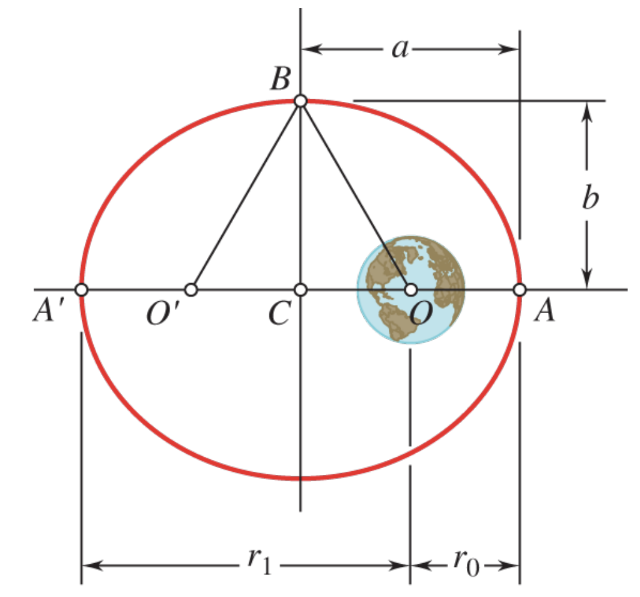
\includegraphics[width=0.4\textwidth]{periodic time.png}
\end{figure}
Time to complete 1 orbit:
\[\tau=\frac{\text{Area of elliptical orbit}}{\text{Areal velocity}}\]
From geometry, the major and minor axes are:
\[a = \frac{1}{2}(r_0 + r_1)\]
\[b = \sqrt{r_0r_1}\]
The area of an ellipse is:
\[A=\pi ab\]
Areal velocity (constant):
\[dA=\frac{1}{2}r^2d\theta\]
\[\frac{dA}{dt}=\frac{1}{2}r^2\frac{d\theta}{dt}=\frac{h}{2} \quad (h=r^2\dot{\theta})\]
Thus periodic time is:
\[\boxed{\tau = \frac{A}{h/2} = \frac{2A}{h} = \frac{2\pi ab}{h}}\] 
\newpage
\begin{center}
    \Large \textbf{Energy}
\end{center}
\makeatletter
\@fleqntrue
\makeatother
\begin{multicols}{2}
\section*{Work}
\[U_{1\to2}=\int_{r_1}^{r_2}\vec{F}\cdot d\vec{r}\]
Constant force in rectilinear motion:
\begin{figure}[H]
    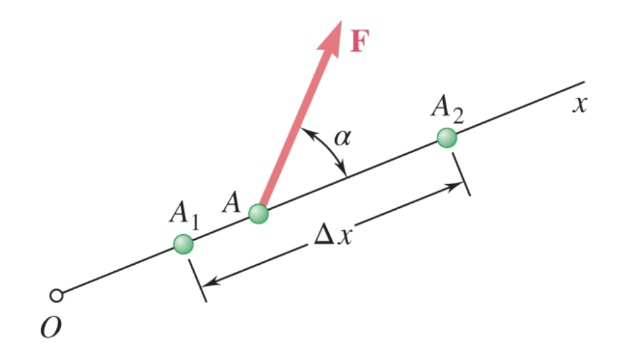
\includegraphics[width=0.3\textwidth]{work.png}
\end{figure}
\[U_{1\to2}=Fcos(\alpha)\Delta x\]
\textbf{Work by gravity/weight}
\[U_{g,1\to2}=-W\Delta y\]
\textbf{Work by gravity (space)}
\[U_{g,1\to2}=\frac{GMm}{r_2}-\frac{GMm}{r_1}\]
\textbf{Work by spring}
\[U_{s,1\to2}=-\frac{1}{2}k(x_2^2-x_1^2)=\frac{1}{2}k(x_1^2-x_2^2)\]
\section*{Work and Energy}
\[U_{1\to2}=T_2-T_1\]
\[T_2=T_1+U_{1\to2}\]
Work of a force = change in kinetic Energy\\
Kinetic energy = capacity to do work\\
\underline{Note:} $T=\frac{1}{2}mv^2$
\section*{Power and Efficiency}
\textbf{Power}
\[P=\frac{dU}{dt}=\vec{F}\cdot\vec{v}\]
\textbf{Efficiency}
\[\eta=\frac{P_{out}}{P_{in}}\]
\section*{Potential Energy}
\textbf{Gravitational Potential}\\
On Earth
\[V_g=Wy=mgh\]
In space
\[V_g=-\frac{GMm}{r}=-\frac{WR^2}{r}\]
\textbf{Elastic Potential}
\[V_e=\frac{1}{2}kx^2\]
\section*{Conservation of Energy}
\[T_1+V_{g1}+V_{e1}+U_{1\to2}^{NC}=T_2+V_{g2}+V_{e2}\]

\end{multicols}
\end{document}
